\section{Implementation and results}
In the previous section, we introduced the Alpha algorithm and taken assumptions which were transformed into a timed automaton. The description provides the details to implement the Alpha algorithm with any suitable tool of choice. In this section, we will focus on implementation with regards to the specific tool of our choice, UPPAAL. UPPAAL is one of the major tools for model checking and verification of real-time systems that can be modeled as timed automata. As the previous section finished on timed automaton, we will start by presenting timed automaton implemented in UPPAAL. We will draw connections between them as presented in Figure \ref{fig:automaton} and Figure \ref{fig:automaton_uppaal}. Then, we will explain global functions and state.

\begin{figure}[H]
\caption{UPPAAL implementation of the timed automaton}
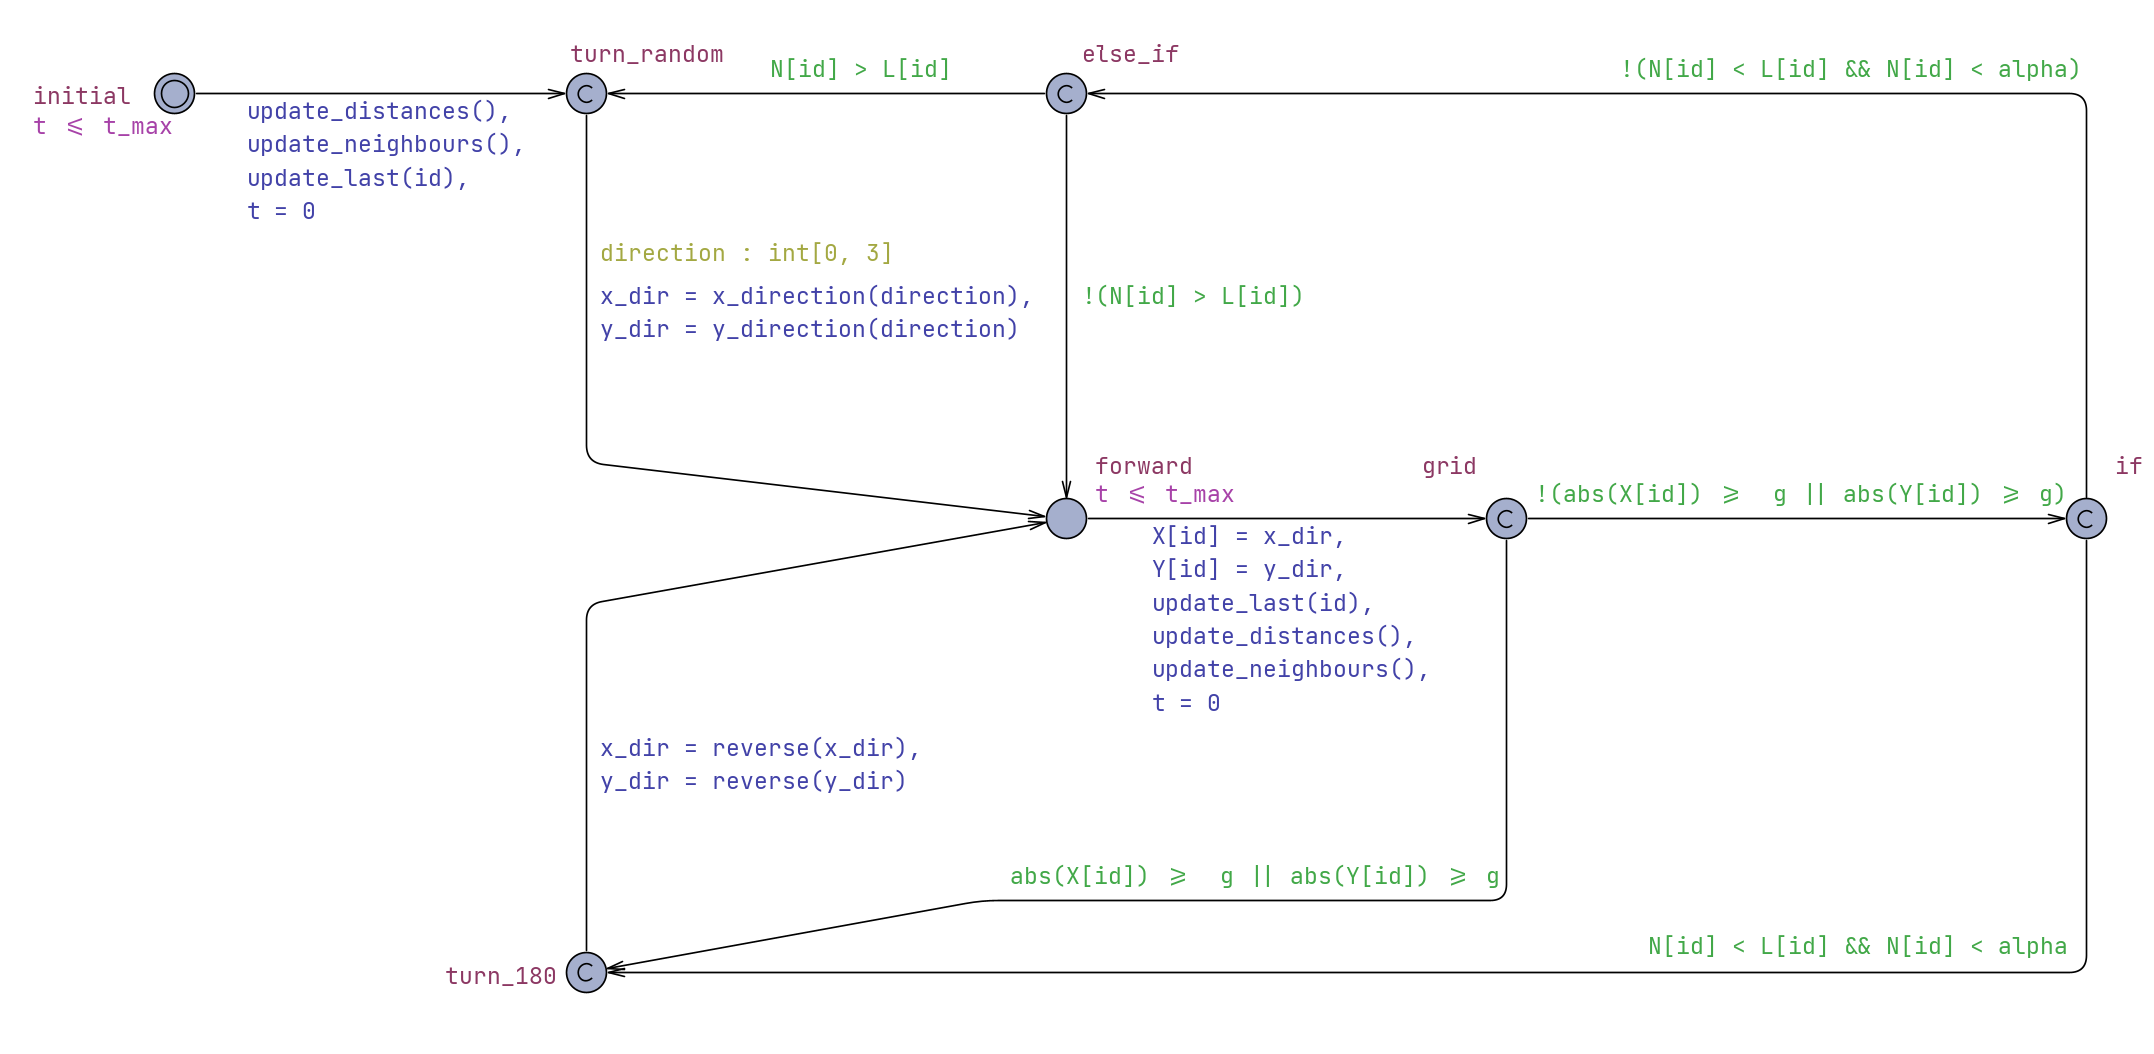
\includegraphics[width=\textwidth]{images/automaton_uppaal.png}
\label{fig:automaton_uppaal}
\end{figure}

\noindent
Variables of the timed automaton presented in Figure \ref{fig:automaton_uppaal}:\\
\textbf{id} - unique identifier of the robot;\\
\textbf{x\_dir} - horizontal direction component;\\
\textbf{y\_dir} - vertical direction component;\\
\textbf{alpha} - alpha parameter;\\
\textbf{g} - grid boundary parameter;\\
\textbf{t\_max} - time threshold for inactivity;\\\\
\noindent
To start with comparison between general automaton and its specific implementation in UPPAAL, let us notice that both automata have the same set of states and transitions apart from the additional state \textbf{grid} that limits the robots environment. Guarded transitions use the same conditions. Each robot accesses its own set of condition variables by providing \textbf{id} to the global arrays. Array \textbf{N} holds the number of neighbours for each robot. Array \textbf{L} holds the last number of neighbours for each robot. Those variables are held in the global arrays so that a single robot could update the number of neighbours for all of the other robots every time it moves. It may seem counter intuitive that a single robot updates the variables of other robots. However, the execution of the system composed from multiple robots is based on interleavings. At any given time a single robot transitions between states. This means that only the moving robot is guaranteed to have true information about number of connections. Global updates of the number of neighbours is a way to mimic physical, continuous signal that would determine whether robots are connected or not. It eliminates the situation where robot would make a decision on already outdated information. The implementation assumes that each time a robot moves it will update its coordinates, update the last number of neighbours for itself and update the current number of neighbours for all robots. Use of the coordinates is necessary as the state of connection is determined by the Euclidean distance between robots and radius of the assumed communication technology. The update of the number of neighbours is achieved by calling \textbf{update\_last(id)} and \textbf{update\_neighbours()}. Figure \ref{fig:neighbours} shows the process of updating the number of connections for all robots.

\begin{figure}[H]
\caption{Implementation of \textbf{update\_neighbours()} and \textbf{neighbours()}}
\lstset { language=C++ }
\begin{lstlisting}
int neighbours(int id){
    // returns the number of connections for a robot with a given id
    int x = X[id];  // x coordinate
    int y = Y[id];  // y coordinate
    int k = 0;      // neighbour counter k
    int i = 0;   
    for (i = 0; i < n; i++){
        double d = distance(x, y, X[i], Y[i]);
        bool c = connected(d);
        // is robot connected to another robot
        if(i != id && c){
            k++;
        }
    }
    return k;
}

void update_neighbours(){
    // updates the array that stores number of neighbours for each robot
    int i;
    for (i = 0; i < n; i++){
        N[i] = neighbours(i);
    }
}
\end{lstlisting}
\label{fig:neighbours}
\end{figure}
\noindent
The number of connections will then determine the next transitions. Transition that is forced by the clock in the \textbf{forward} state will always result in the robot moving by a unit step in its current direction. Then, based on logical value of the conditions guarding transitions, it can also change its direction. The direction will change after robot reaches and transitions from states \textbf{turn\_random} or \textbf{turn\_180}. Additonally, robot will perform the 180 degree turn if it reaches the boundary of the grid that is its environment. The random turn is realised as a random choice between four directions: up, right, down, up and translating it into x, y coordinates. The 180 degree turn is realised as choosing the opposite direction to the current one. Change of direction is achieved by functions \textbf{x\_direction(direction)}, \textbf{y\_direction(direction)}, \textbf{reverse(direction)}. Figure \ref{fig:direction} show the process of changing direction.
\begin{figure}[H]
\caption{Implementation of \textbf{x\_direction(direction)} and \textbf{reverse(direction)}}
\lstset { language=C++ }
\begin{lstlisting}
int x_direction(int direction){
    // maps direction to x axis
    if (direction == 1){
        // right
        return 1;
    }
    if (direction == 3){
        // left
        return -1;
    }
    // neither
    return 0;
}

int reverse(int direction){
    // reverses direction
    return direction * -1;
}
\end{lstlisting}
\label{fig:direction}
\end{figure}
\noindent
The last element of the implementation is time. Each robot has its own clock that limits how long it can stay in the states with defined invariants: \textbf{initial}, \textbf{forward}. After transitioning from those states, a robot will reset its clock. Only in those states, the time passes. Other states are so called committed locations. In committed locations time does not pass which means that individual robot clocks do not progress. As a consequence the time progresses during the forward motion of the robot but decision to turn happens instantaneously.

The implementation of the Alpha algorithm in UPPAAL and the presented timed automaton model depct the behavior of a single robot. In order to create a robot swarm we need to instantiate multiple such robots and compose them into a system. This is achieved in UPPAAL with code presented in Figure \ref{fig:composition}.
\begin{figure}[H]
\caption{System consisting of two models in UPPAAL}
\lstset { language=C++ }
\begin{lstlisting}
// int id, int x, int y, int x_dir, int y_dir
P1 = Robot(0, 0, 0, 0, 0);
P2 = Robot(1, 0, 0, 0, 0);
system P1, P2;
\end{lstlisting}
\label{fig:composition}
\end{figure}

\noindent
The created system is parameterised with the variables, presented in Figure \ref{fig:parameters}. Variable \textbf{r} is a radius of the the simulated communication technology. If the Euclidean distance between robots is smaller than \textbf{r}, the robots are in range and therefore connected. Variable \textbf{g} establishes the boundaries of the grid in which robots move. Dimensions of the grid are 2\textbf{g} $\times$ 2\textbf{g} with center at (\textbf{x}$=0, $\textbf{y}$=0$). Variable \textbf{alpha} is an alpha parameter of the implemented algorithm. Variable \textbf{t\_max} is the maximum time a robot can remain in a state with a defined invariant. To reiterate, the system is composed from two robots implementing the Alpha algorithm, which move on 10$\times$10 grid, with alpha parameter equal to one, radius of the connectivity equal to two and with time limit equal to five.

\begin{figure}[H]
\caption{System parameters}
\lstset { language=C++ }
\begin{lstlisting}
const int r = 2;
const int g = 5;
const int alpha = 1;
const int t_max = 5
\end{lstlisting}
\label{fig:parameters}
\end{figure}

\noindent
To examine the correctness of the implemented model presented in Figure \ref{fig:automaton_uppaal} we successfully verified following properties of the system parameterised with variables from Figure \ref{fig:parameters}.\\\\
Verified properties:\\
1. \texttt{A[] not deadlock}\\
2. \texttt{A[] N[0] == N[1]}\\
3. \texttt{A[] P1.forward or P1.initial imply P1.t <= t\_max}\\
4. \texttt{A[] not P1.initial and not P1.forward imply P1.t == 0}\\
5. \texttt{A[] P1.turn\_random imply P2.initial or P2.forward}\\
6. \texttt{A[] P1.forward imply (P1.x\_dir != 0 and P1.y\_dir == 0) or (P1.x\_dir == 0 and P1.y\_dir != 0)}\\\\
Explanation of verified properties:\\
1. For all paths of the system there is never a deadlock.\\
2. For all paths of the system number of neighbours of one robot is always equal to the number of neighbours of the second robot. Communication realised by sharing global state that is updated by the global function, is correctly implemented. Information about the number of neighbours is updated for both robots at the same time.\\
3. For all paths of the system, invariant on location \textbf{forward} and \textbf{initial} is obeyed.\\
4. For all paths of the system, time does not progress outside of locations \textbf{initial} and \textbf{forward}.\\
5. For all paths of the system, if first robot is in the location \textbf{turn\_random} then the other robot must be either in location \textbf{initial} or \textbf{forward}. Sequence of locations of type committed cannot be interleaved by another robot.\\
6. For all paths of the system, robot in location \textbf{forward} has either set only horizontal direction or vertical. Robot will move only up, down, left or right. Robot will never move diagonally or move without horizontal and vertical direction.\\\\
\noindent
We started from general timed automaton implementing the Alpha algorithm. We implemented it using UPPAAL and recreated states, transitions and conditions. We explained the reasoning behind using the global state for condition variables and the mechanism of updating them. We showed how the robot movement and changes of directions are realised and when it happens. We described the timing aspect and its practical implications on the behaviour of the model. We showed how a system is created and parameterised. Finally, we successfully verified properties that increase the probability of correct implementation of the Alpha algorithm in robot swarm.